\documentclass[tikz,border=2pt]{standalone}
\usepackage{amsmath,amssymb}
\usetikzlibrary{arrows.meta}
\begin{document}
% Base-stock policy, S = 5, lead time l = 1, demands 2,3,1,4,0,3,2,5,1,2 in periods 1..10.
% At the start of period k the inventory level I_k (blue) plus the quantity on order Q_k (red)
% equals the inventory position P_k = S = 5, and the order Q_k = D_{k-1} replaces last period's demand.
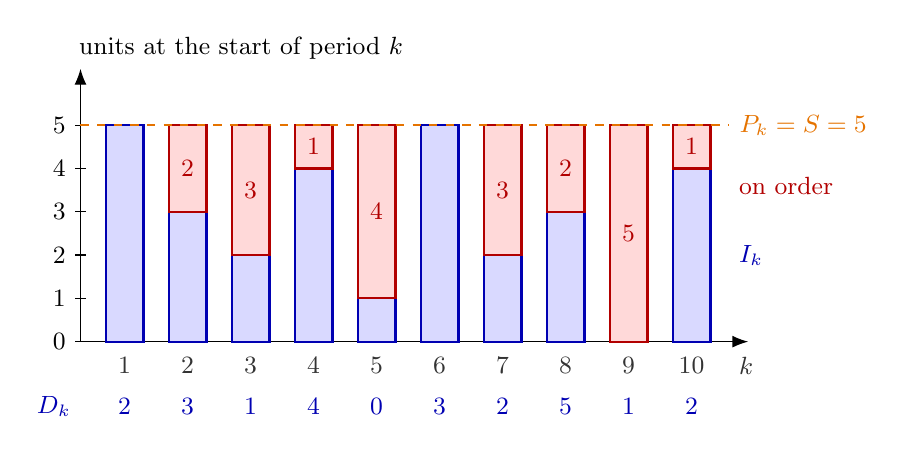
\begin{tikzpicture}[font=\small, >={Latex[length=2mm]}, x=0.8cm, y=0.55cm]
  \draw[->] (0.3,0) -- (10.9,0);
  \draw[->] (0.3,0) -- (0.3,6.3) node[anchor=south west, xshift=-4pt] {units at the start of period $k$};
  \foreach \v in {0,1,2,3,4,5} {\draw (0.38,\v) -- (0.22,\v) node[left] {$\v$};}
  \foreach \k/\i/\q in {1/5/0,2/3/2,3/2/3,4/4/1,5/1/4,6/5/0,7/2/3,8/3/2,9/0/5,10/4/1} {
    \ifnum\i>0 \fill[blue!15] (\k-0.3,0) rectangle (\k+0.3,\i); \draw[blue!70!black, thick] (\k-0.3,0) rectangle (\k+0.3,\i); \fi
    \ifnum\q>0 \fill[red!15] (\k-0.3,\i) rectangle (\k+0.3,5); \draw[red!70!black, thick] (\k-0.3,\i) rectangle (\k+0.3,5);
      \node[red!70!black] at (\k,{(\i+5)/2}) {$\q$}; \fi
    \node[gray!40!black] at (\k,-0.55) {$\k$};
  }
  \draw[orange!90!black, thick, dashed] (0.3,5) -- (10.6,5) node[right] {$P_k=S=5$};
  \node[gray!40!black, anchor=west] at (10.6,-0.55) {$k$};
  % demand row
  \node[blue!70!black, anchor=east] at (0.3,-1.5) {$D_k$};
  \foreach \k/\d in {1/2,2/3,3/1,4/4,5/0,6/3,7/2,8/5,9/1,10/2} {\node[blue!70!black] at (\k,-1.5) {$\d$};}
  % legend by direct labels
  \node[blue!70!black, anchor=west] at (10.6,2) {$I_k$};
  \node[red!70!black, anchor=west] at (10.6,3.6) {on order};
\end{tikzpicture}
\end{document}
